\section{Reward}
something about the reward in general with ref to theory chapter

\subsection*{First reward function}
The first reward function, that is used in this project is the reward function from the paper \cite{DBLP:journals/corr/LillicrapHPHETS15}: \\
\textit{"For the Torcs environment we used a reward function which provides a positive reward each step for the velocity of the car projected along the direction and a penalty of -1 for collisions. Episodes were terminated if progress was not made along the track after 500 frames.}\\
To understand this a figure to illustrate the reward can be seen on \Cref{fig:Reward_paper}.

\begin{figure}[H]
	\centering
	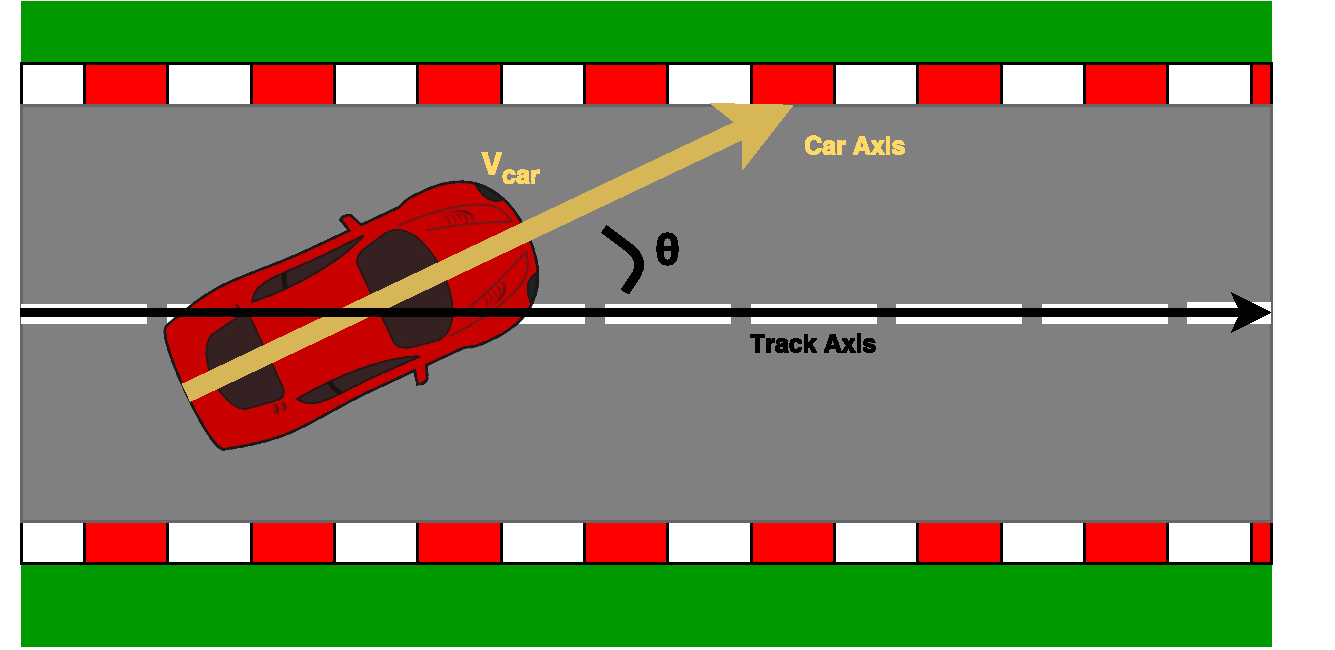
\includegraphics[width=1\textwidth]{Figures/Result/Reward_paper.pdf}
	\caption{Explanation of the reward used in the paper \cite{DBLP:journals/corr/LillicrapHPHETS15} }
	\label{fig:Reward_paper}
\end{figure}

The reward function is then:
\begin{equation}
Reward = V_{car} \cdot cos(\theta) 
\end{equation}
The idea this reward function uses it it gets an reward for how fast the car drives in the center of the track. The agent gets more reward, when the car is driving fast at the center of the track, and less reward when the car is driving fast away from the center of the track. 

The reward is added to the total reward after every step. The total reward will then be the reward when an episode is finish. An episode is ended when the car is out of track, the car is driving backwards or the car has finished a track. 

The result of this reward function can be seen on the graph below. 

Here it is seen that this reward didn't have the wanted effect, where the reward conjugate at the maximum. By looking at the simulator, it looks like the car is not finding the center of the track, it will then hit an edge an the episode is terminated. Therefore, the neural network stuck in a poor local minimum.  

\subsection*{Second reward function}
After using the first reward function it was concluded that this reward function didn't perform as expected. Because the reward function is important for learning, another reward function is tried. This reward function is taken from the blog \cite{DDPG_Torcs}. Here it uses the same idea, that the reward should be bigger if the car drives fast in the center of the track, and less reward when it is far away from the center. The reward function looks like this:

\begin{equation}
Reward = V_{car} \cdot cos(\theta) - V_{car} \cdot sin(\theta) - V_{car} \cdot \mid trackPos\mid 
\end{equation}
The TrackPos gives percent the car is off center of track. Which is useful in this reward function, when it is wished the car is near the center.  

In this equation the first term want to maximum longitudinal velocity, second term try to minimize transverse velocity, and then it also penalize the AI if it constantly drives very off center of the track in the third term.

Here we see the agent learns how to drive, and this is the reward function where the best results came in this project. It improves the learning time and the stability of the training. 